\documentclass[a4paper,12pt]{article}
\usepackage[colorlinks,
    citecolor=black,
    filecolor=black,
    linkcolor=black,
    urlcolor=black]{hyperref}
   
\usepackage{polski}
\usepackage[utf8]{inputenc}
\usepackage{amsmath}
\usepackage{graphicx}
\usepackage[colorinlistoftodos]{todonotes}
\usepackage{amssymb}
\usepackage[a4paper, total={6in, 9in}]{geometry}
\usepackage{float}
\usepackage{setspace}
\usepackage{caption}

\title{Lorem Ipsum}

\author{Julianna Mikucka}
\date{\today}

\begin{document}
\maketitle
\setcounter{tocdepth}{2} %shows all levels incl. paragraph

\begin{flushleft}

\tableofcontents
\end{flushleft}

\newpage


\section{\textbf{Lorem Ipsum}}

Lorem ipsum dolor sit amet, consectetur adipiscing elit. Cras est ligula, consequat non dignissim quis, bibendum eu diam. Mauris finibus, mauris vel tincidunt efficitur, ligula leo tempus lacus, ac euismod tellus odio sit amet risus. Ut vestibulum convallis neque eget feugiat. Etiam interdum tellus nulla, at aliquam mi commodo et. Proin vehicula dictum erat, sit amet accumsan felis hendrerit vitae. Nulla ornare eget libero ut rutrum. Cras aliquam risus at auctor iaculis. Aliquam lorem metus, aliquet in cursus sed, tristique in velit. Nulla tincidunt congue ligula eget scelerisque. Nam vestibulum sem rhoncus quam lacinia, a ultricies sapien convallis. Nullam sed vestibulum eros, in sodales magna. Ut urna justo, ultricies at lacinia at, dapibus at leo. Aliquam iaculis nunc est, egestas imperdiet diam faucibus sit amet. Donec urna mi, pellentesque ut dolor nec, dignissim aliquet tellus. Sed id pretium nisi. \todo[color=pink!40]{Aliquam iaculis nunc est, egestas imperdiet diam faucibus sit amet.}Aliquam lorem metus, aliquet in cursus sed, tristique in velit. Nulla tincidunt congue ligula eget scelerisque. Nam vestibulum sem rhoncus quam lacinia, a ultricies sapien convallis. \ref{fig:lorem}. 

\begin{figure}[h!]
\centering 

\includegraphics[width=0.8\textwidth]{loremipsum.jpg}
\caption{\label{fig:lorem}}
\end{figure}

\section{Z czym to się je?}

\subsection{Czym jest Lorem Ipsum?}

Lorem Ipsum\footnote{Pellentesque viverra porta mi, ac accumsan nibh congue at. Quisque dictum congue nibh in mattis. Mauris eros odio, commodo ac aliquam et, ultrices eu nunc.} jest tekstem stosowanym jako przykładowy wypełniacz w przemyśle poligraficznym. Został po raz pierwszy użyty w XV w. przez nieznanego drukarza do wypełnienia tekstem próbnej książki. Pięć wieków później zaczął być używany przemyśle elektronicznym, pozostając praktycznie niezmienionym. Spopularyzował się w latach 60. XX w. wraz z publikacją arkuszy Letrasetu, zawierających fragmenty Lorem Ipsum, a ostatnio z zawierającym różne wersje Lorem Ipsum oprogramowaniem przeznaczonym do realizacji druków na komputerach osobistych, jak Aldus PageMaker

\subsection{Do czego tego użyc?}

Ogólnie znana teza głosi, iż użytkownika może rozpraszać zrozumiała zawartość strony, kiedy ten chce zobaczyć sam jej wygląd. Jedną z mocnych stron używania Lorem Ipsum jest to, że ma wiele różnych „kombinacji” zdań, słów i akapitów, w przeciwieństwie do zwykłego: „tekst, tekst, tekst”, sprawiającego, że wygląda to „zbyt czytelnie” po polsku. Wielu webmasterów i designerów używa Lorem Ipsum jako domyślnego modelu tekstu i wpisanie w internetowej wyszukiwarce ‘lorem ipsum’ spowoduje znalezienie bardzo wielu stron, które wciąż są w budowie. Wiele wersji tekstu ewoluowało i zmieniało się przez lata, czasem przez przypadek, czasem specjalnie (humorystyczne wstawki itd).

\begin{itemize}
\item Nam - id odio orci.
\item[$\square$] Curabitur  - semper consectetur erat non ullamcorper.
\item Nulla - at sapien ornare, imperdiet augue quis, pharetra leo.
\item[$\square$] Vestibulum - ante ipsum primis in faucibus orci luctus et ultrices posuere
\item Mauris - eros odio, commodo ac aliquam et, ultrices eu nunc. 
\item[$\square$] Sed - id erat et est faucibus accumsan.

\end{itemize}

\subsection{Skąd to się wzięło?}

W przeciwieństwie do rozpowszechnionych opinii, Lorem Ipsum\footnote{liquam gravida, lectus sed semper consectetur, lacus nunc volutpat arcu, at maximus leo elit quis velit.} nie jest tylko przypadkowym tekstem. Ma ono korzenie w klasycznej łacińskiej literaturze z 45 roku przed Chrystusem, czyli ponad 2000 lat temu! Richard McClintock, wykładowca łaciny na uniwersytecie Hampden-Sydney w Virginii, przyjrzał się uważniej jednemu z najbardziej niejasnych słów w Lorem Ipsum – consectetur – i po wielu poszukiwaniach odnalazł niezaprzeczalne źródło: Lorem Ipsum pochodzi z fragmentów (1.10.32 i 1.10.33) „de Finibus Bonorum et Malorum”, czyli „O granicy dobra i zła”, napisanej właśnie w 45 p.n.e. przez Cycerona. Jest to bardzo popularna w czasach renesansu rozprawa na temat etyki. Pierwszy wiersz Lorem Ipsum, „Lorem ipsum dolor sit amet...” pochodzi właśnie z sekcji 1.10.32.

Standardowy blok Lorem Ipsum, używany od XV wieku, jest odtworzony niżej dla zainteresowanych. Fragmenty 1.10.32 i 1.10.33 z „de Finibus Bonorum et Malorum” Cycerona, są odtworzone w dokładnej, oryginalnej formie, wraz z angielskimi tłumaczeniami H. Rackhama z 1914 roku.

\begin{figure}[h!]
\centering 

\includegraphics[width=0.8\textwidth]{emot2.png}
\caption{\label{fig:emot}}
\end{figure}

\begin{enumerate}
\item Lorem Ipsum:
\begin{itemize}
\item  Proin tellus risus, condimentum a pulvinar ac, varius vel dui.
\item[--] Mauris at tincidunt elit. 
\end{itemize}
\item Curabitur:
\begin{description}
\item[Sed] id erat et est faucibus accumsan.
\item[Vestibulum] rhoncus ante in nisi consectetur luctus vitae sollicitudin odio.
\end{description}
\end{enumerate}

\subsection{Skąd to wziąć?}

Jest dostępnych wiele różnych wersji Lorem Ipsum\footnote{Curabitur semper consectetur erat non ullamcorper. Nulla at sapien ornare, imperdiet augue quis, pharetra leo.}, ale większość zmieniła się pod wpływem dodanego humoru czy przypadkowych słów, które nawet w najmniejszym stopniu nie przypominają istniejących. Jeśli masz zamiar użyć fragmentu Lorem Ipsum, lepiej mieć pewność, że nie ma niczego „dziwnego” w środku tekstu. Wszystkie Internetowe generatory Lorem Ipsum mają tendencje do kopiowania już istniejących bloków, co czyni nasz pierwszym prawdziwym generatorem w Internecie. Używamy zawierającego ponad 200 łacińskich słów słownika, w kontekście wielu znanych sentencji, by wygenerować tekst wyglądający odpowiednio. To wszystko czyni „nasz” Lorem Ipsum wolnym od powtórzeń, humorystycznych wstawek czy niecharakterystycznych słów.

\begin{tabular}{|p{4.7cm}|} \hline
Donec suscipit placerat ligula, et sagittis nisl aliquam ac. Phasellus sollicitudin.\\ \hline
\end{tabular}

\section{Pozostałe}

\subsection{Curabitur semper consectetur erat non ullamcorper.}

Sed id erat et est faucibus accumsan. Vestibulum rhoncus ante in nisi consectetur luctus vitae sollicitudin odio. Class aptent taciti sociosqu ad litora torquent per conubia nostra, per inceptos himenaeos. Donec a laoreet quam. Curabitur ultricies venenatis urna tincidunt aliquet. Mauris ultricies blandit orci, quis imperdiet mauris facilisis eu. Mauris nulla ante, vestibulum eget facilisis ac, varius id eros. Sed dignissim tincidunt massa, eu tempus lectus. Suspendisse efficitur justo eget ligula sollicitudin tempor in vel lectus. Donec suscipit placerat ligula, et sagittis nisl aliquam ac. Phasellus sollicitudin, velit ac interdum rhoncus, tellus dui pulvinar nulla, sit amet lobortis lacus neque non dolor. Fusce ac lobortis metus. Vestibulum molestie vehicula ipsum ut mollis. Maecenas leo nisl, condimentum id rhoncus non, feugiat eget urna. Pellentesque scelerisque dapibus tellus a fringilla. 

\begin{tabular}{c r @{,} l}
Wyrażenie &
\multicolumn{2}{c}{Wartość}\\ \hline
$\pi$ & 3&1416 \\
$\pi^{\pi}$ & 36&46 \\
$(\pi^{\pi})^{\pi}$ & 80662&7 \\
\end{tabular}


\begin{tabular}{|r|l|} \hline
7C0 & heksadecymalnie \\
3700 & oktalnie \\
11111000000 & binarnie \\
\hline \hline
1984 & dziesietnie \\ \hline
\end{tabular}

\subsection{Quisque ut porta enim, ac congue nisi.}
Lorem
$$ a^{2} $$
Ipsum
\[ a^{2} \]
Curabitur
\begin{displaymath}
c^{2}=a^{2}+b^{2}
\end{displaymath}
Semper
\begin{equation}
\epsilon > 0 \label{eq:eps}
\end{equation}
Ze wzoru (\ref{eq:eps}) otrzymujemy \ldots


$\lim_{n \to \infty}
\sum_{k=1}^n \frac{1}{k^2}
= \frac{\pi^2}{6}$
\\ \\
$$
\lim_{n \to \infty}
\sum_{k=1}^n \frac{1}{k^2}
= \frac{\pi^2}{6}
$$



\subsection{Nam id odio orci.}

Nam id odio orci. Praesent ullamcorper eros in dignissim vestibulum. Nulla facilisi. Duis efficitur euismod nulla, eget varius magna accumsan sit amet. Vivamus quis tempor purus, et iaculis libero. Ut mattis varius est vel ultricies. Nam id ante nisi. Phasellus sed dolor vitae elit efficitur sollicitudin. Nulla consequat euismod suscipit. Pellentesque ante velit, convallis sed nunc ac, feugiat venenatis odio. Fusce in tortor vitae metus mollis dictum. Quisque metus ex, semper nec molestie non, tincidunt in eros. Mauris ut bibendum urna. Mauris at tincidunt elit. 

Partl~\cite{pa} przedstawi\l \ldots
\begin{thebibliography}{99}
\bibitem{pa} H.~Partl:
\emph{German \TeX},
TUGboat Vol.~9,, No.~1 ('88)
\end{thebibliography}


\begin{table}[h!]
\centering
\begin{tabular}{l|r|r}
 & Lorem & Ipsum \\\hline
Nam & id & orci \\\hline
Nulla &&\\ rehulla & 1 & 0 \\\hline
tellus dui & 0 & 1\\\hline
purrla & duna & vici
\end{tabular}
\caption{\label{tab:widgets}Podsumowanie obydwóch istot.}
\end{table}
\newpage


\subsection{Grafika}

\setlength{\unitlength}{1mm}
\begin{picture}(100, 10)
\put(1,1){\circle{2}}
\put(1,1){\circle{4}}
\put(1,1){\circle{6}}
\put(1,1){\circle{8}}
\put(1,1){\circle{10}}
\put(1,1){\circle{12}}
\put(1,1){\circle{14}}
\put(1,1){\circle{16}}

\end{picture}

\setlength{\unitlength}{0.8cm}
\begin{picture}(6,5)
\thicklines
\put(1,0.5){\line(2,1){3}}
\put(4,2){\line(-2,1){2}}
\put(2,3){\line(-2,-5){1}}
\put(0.65,0.3){$A$}
\put(4.05,1.9){$B$}
\put(1.65,2.95){$C$}
\put(3.1,2.5){$a$}
\put(1.3,1.7){$b$}
\put(2.5,1.05){$c$}
\put(0.3,4){$F=
\sqrt{s(s-a)(s-b)(s-c)}$}
\put(3.5,0.4){$\displaystyle
s:=\frac{a+b+c}{2}$}
\end{picture}

\setlength{\unitlength}{2mm}
\begin{picture}(30,20)
\linethickness{0.075mm}
\multiput(0,0)(1,0){26}%
{\line(0,1){20}}
\multiput(0,0)(0,1){21}%
{\line(1,0){25}}
\linethickness{0.15mm}
\multiput(0,0)(5,0){6}%
{\line(0,1){20}}
\multiput(0,0)(0,5){5}%
{\line(1,0){25}}
\linethickness{0.3mm}
\multiput(5,0)(10,0){2}%
{\line(0,1){20}}
\multiput(0,5)(0,10){2}%
{\line(1,0){25}}
\end{picture}

\subsection{Grafika wektorowa}

\begin{figure}[h!]
\centering 

\includegraphics[width=0.8\textwidth]{wek.jpg}
\caption{\label{fig:wek}}
\end{figure}

\begin{figure}[h!]
\centering 
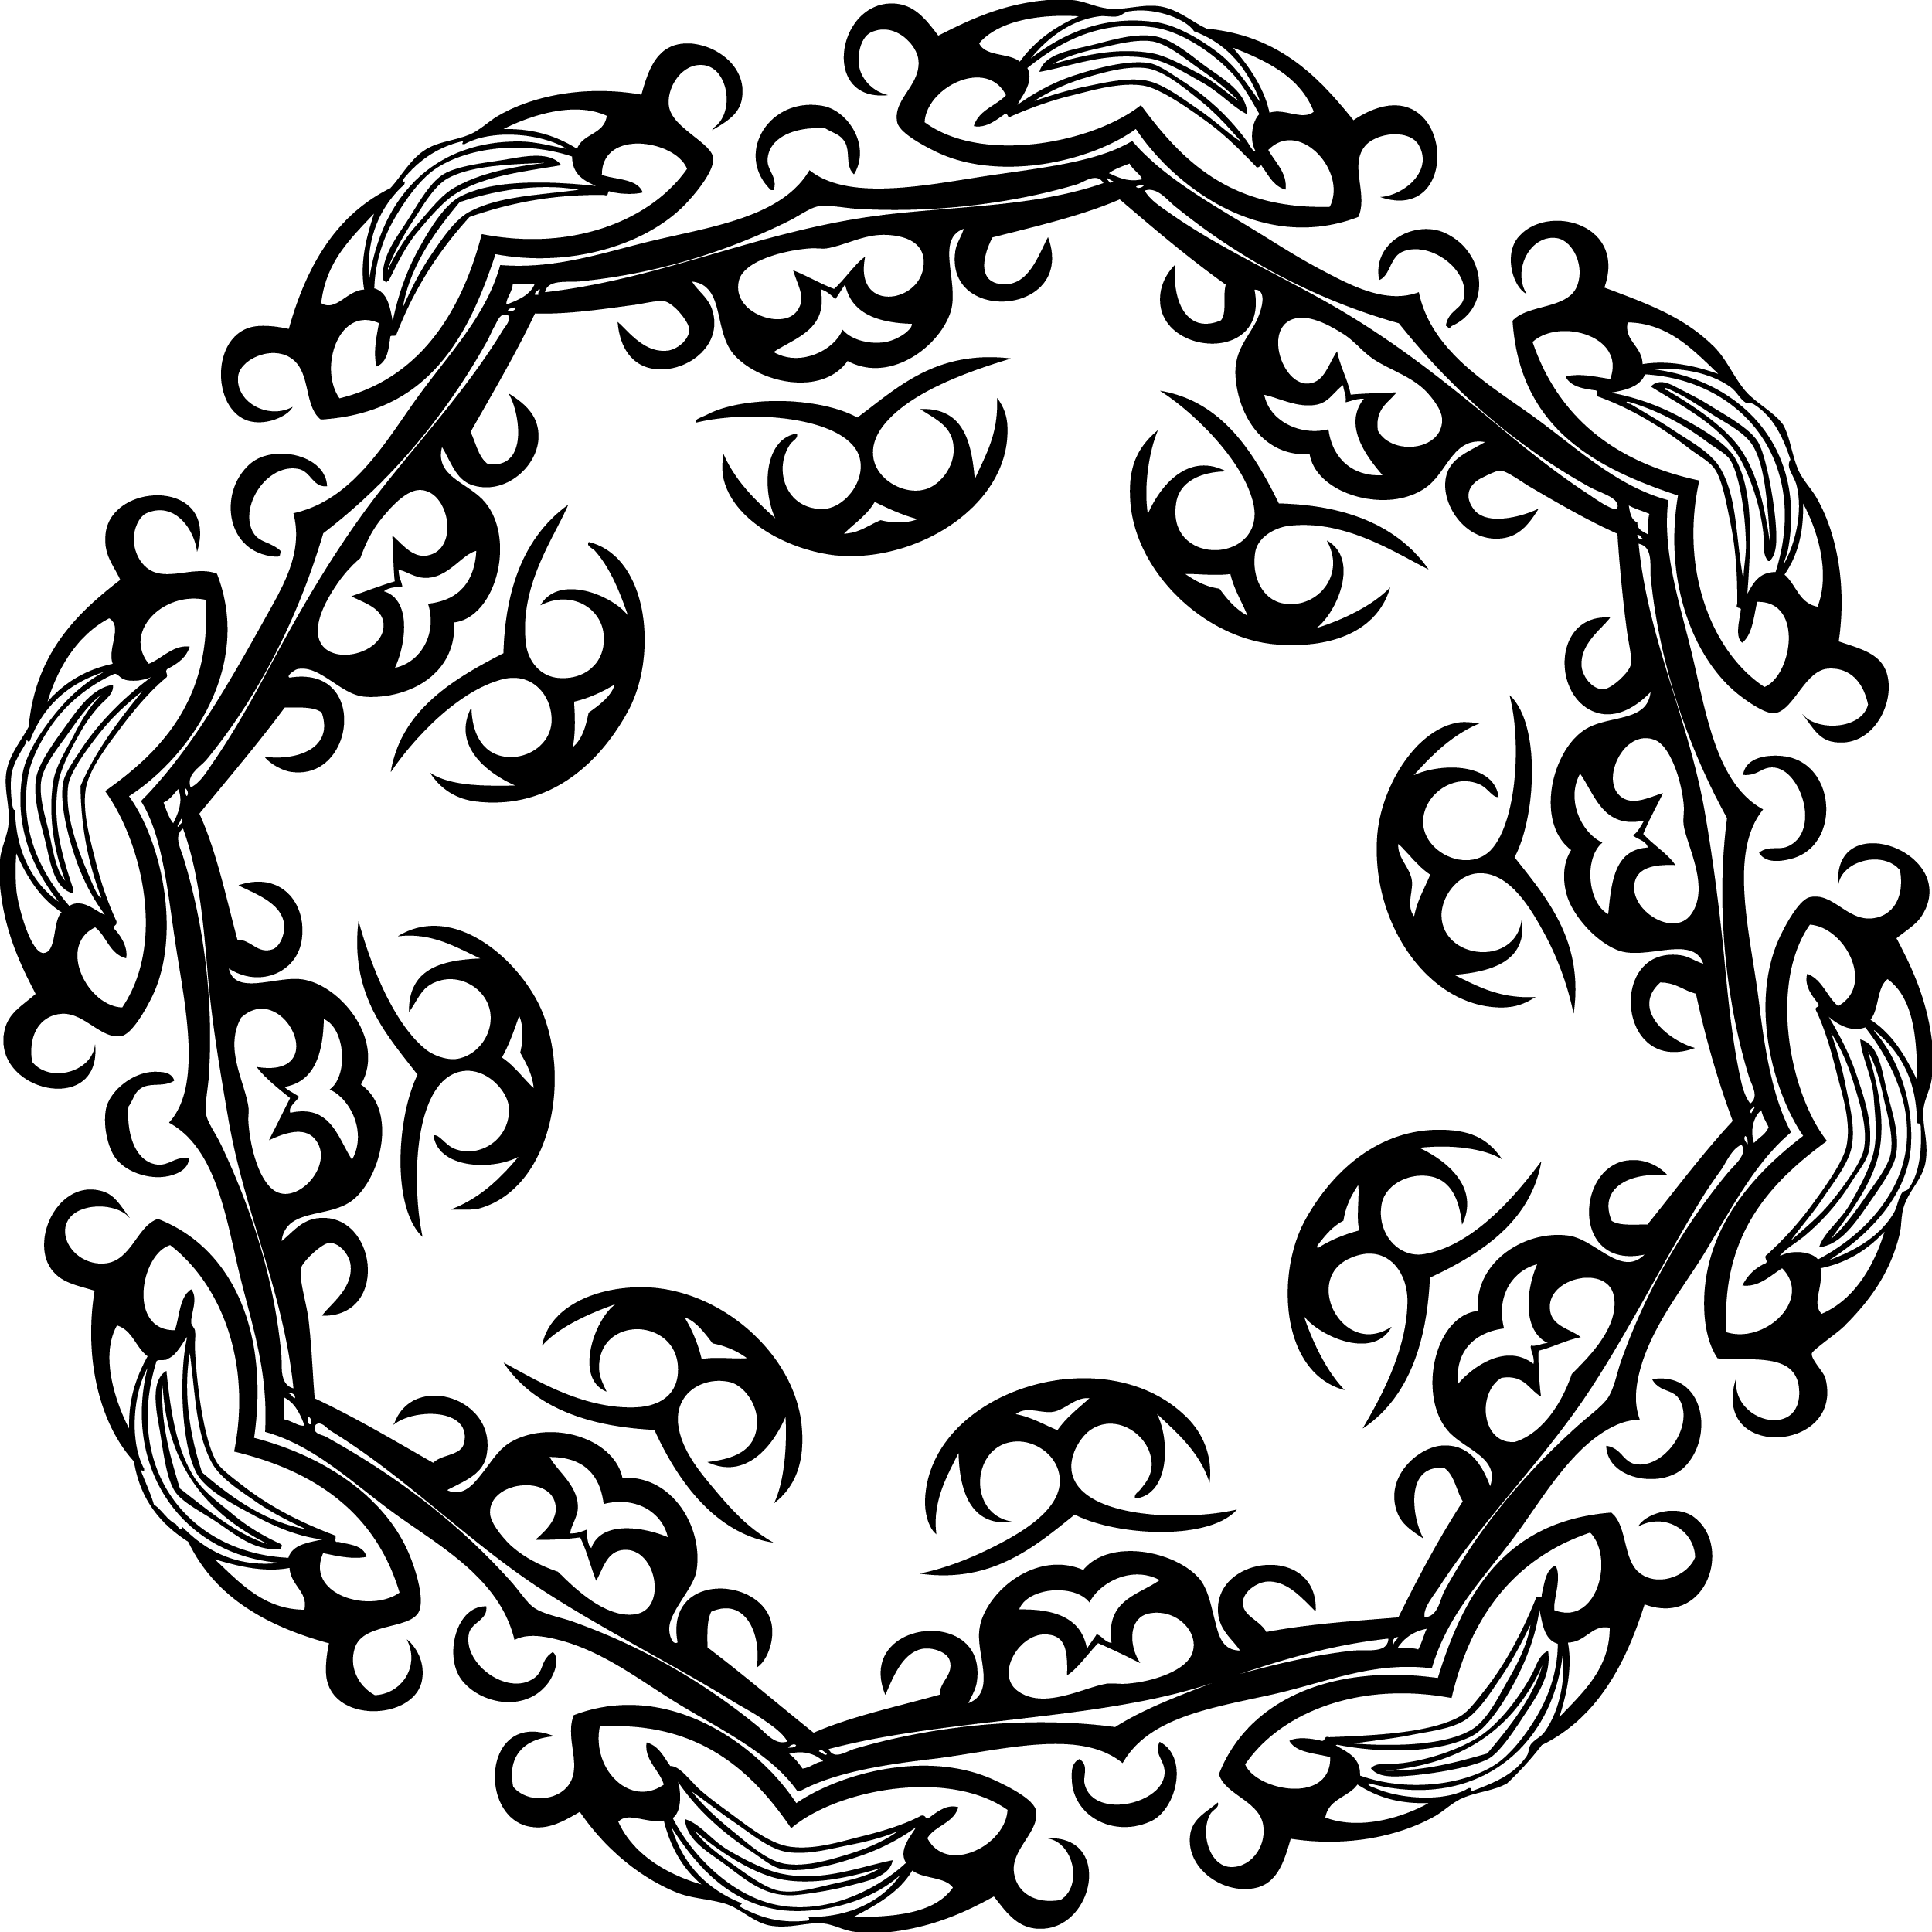
\includegraphics[width=0.8\textwidth]{wektor2.png}
\caption{\label{fig:wekk}}
\end{figure}


\begin{figure}[h!]
\centering 
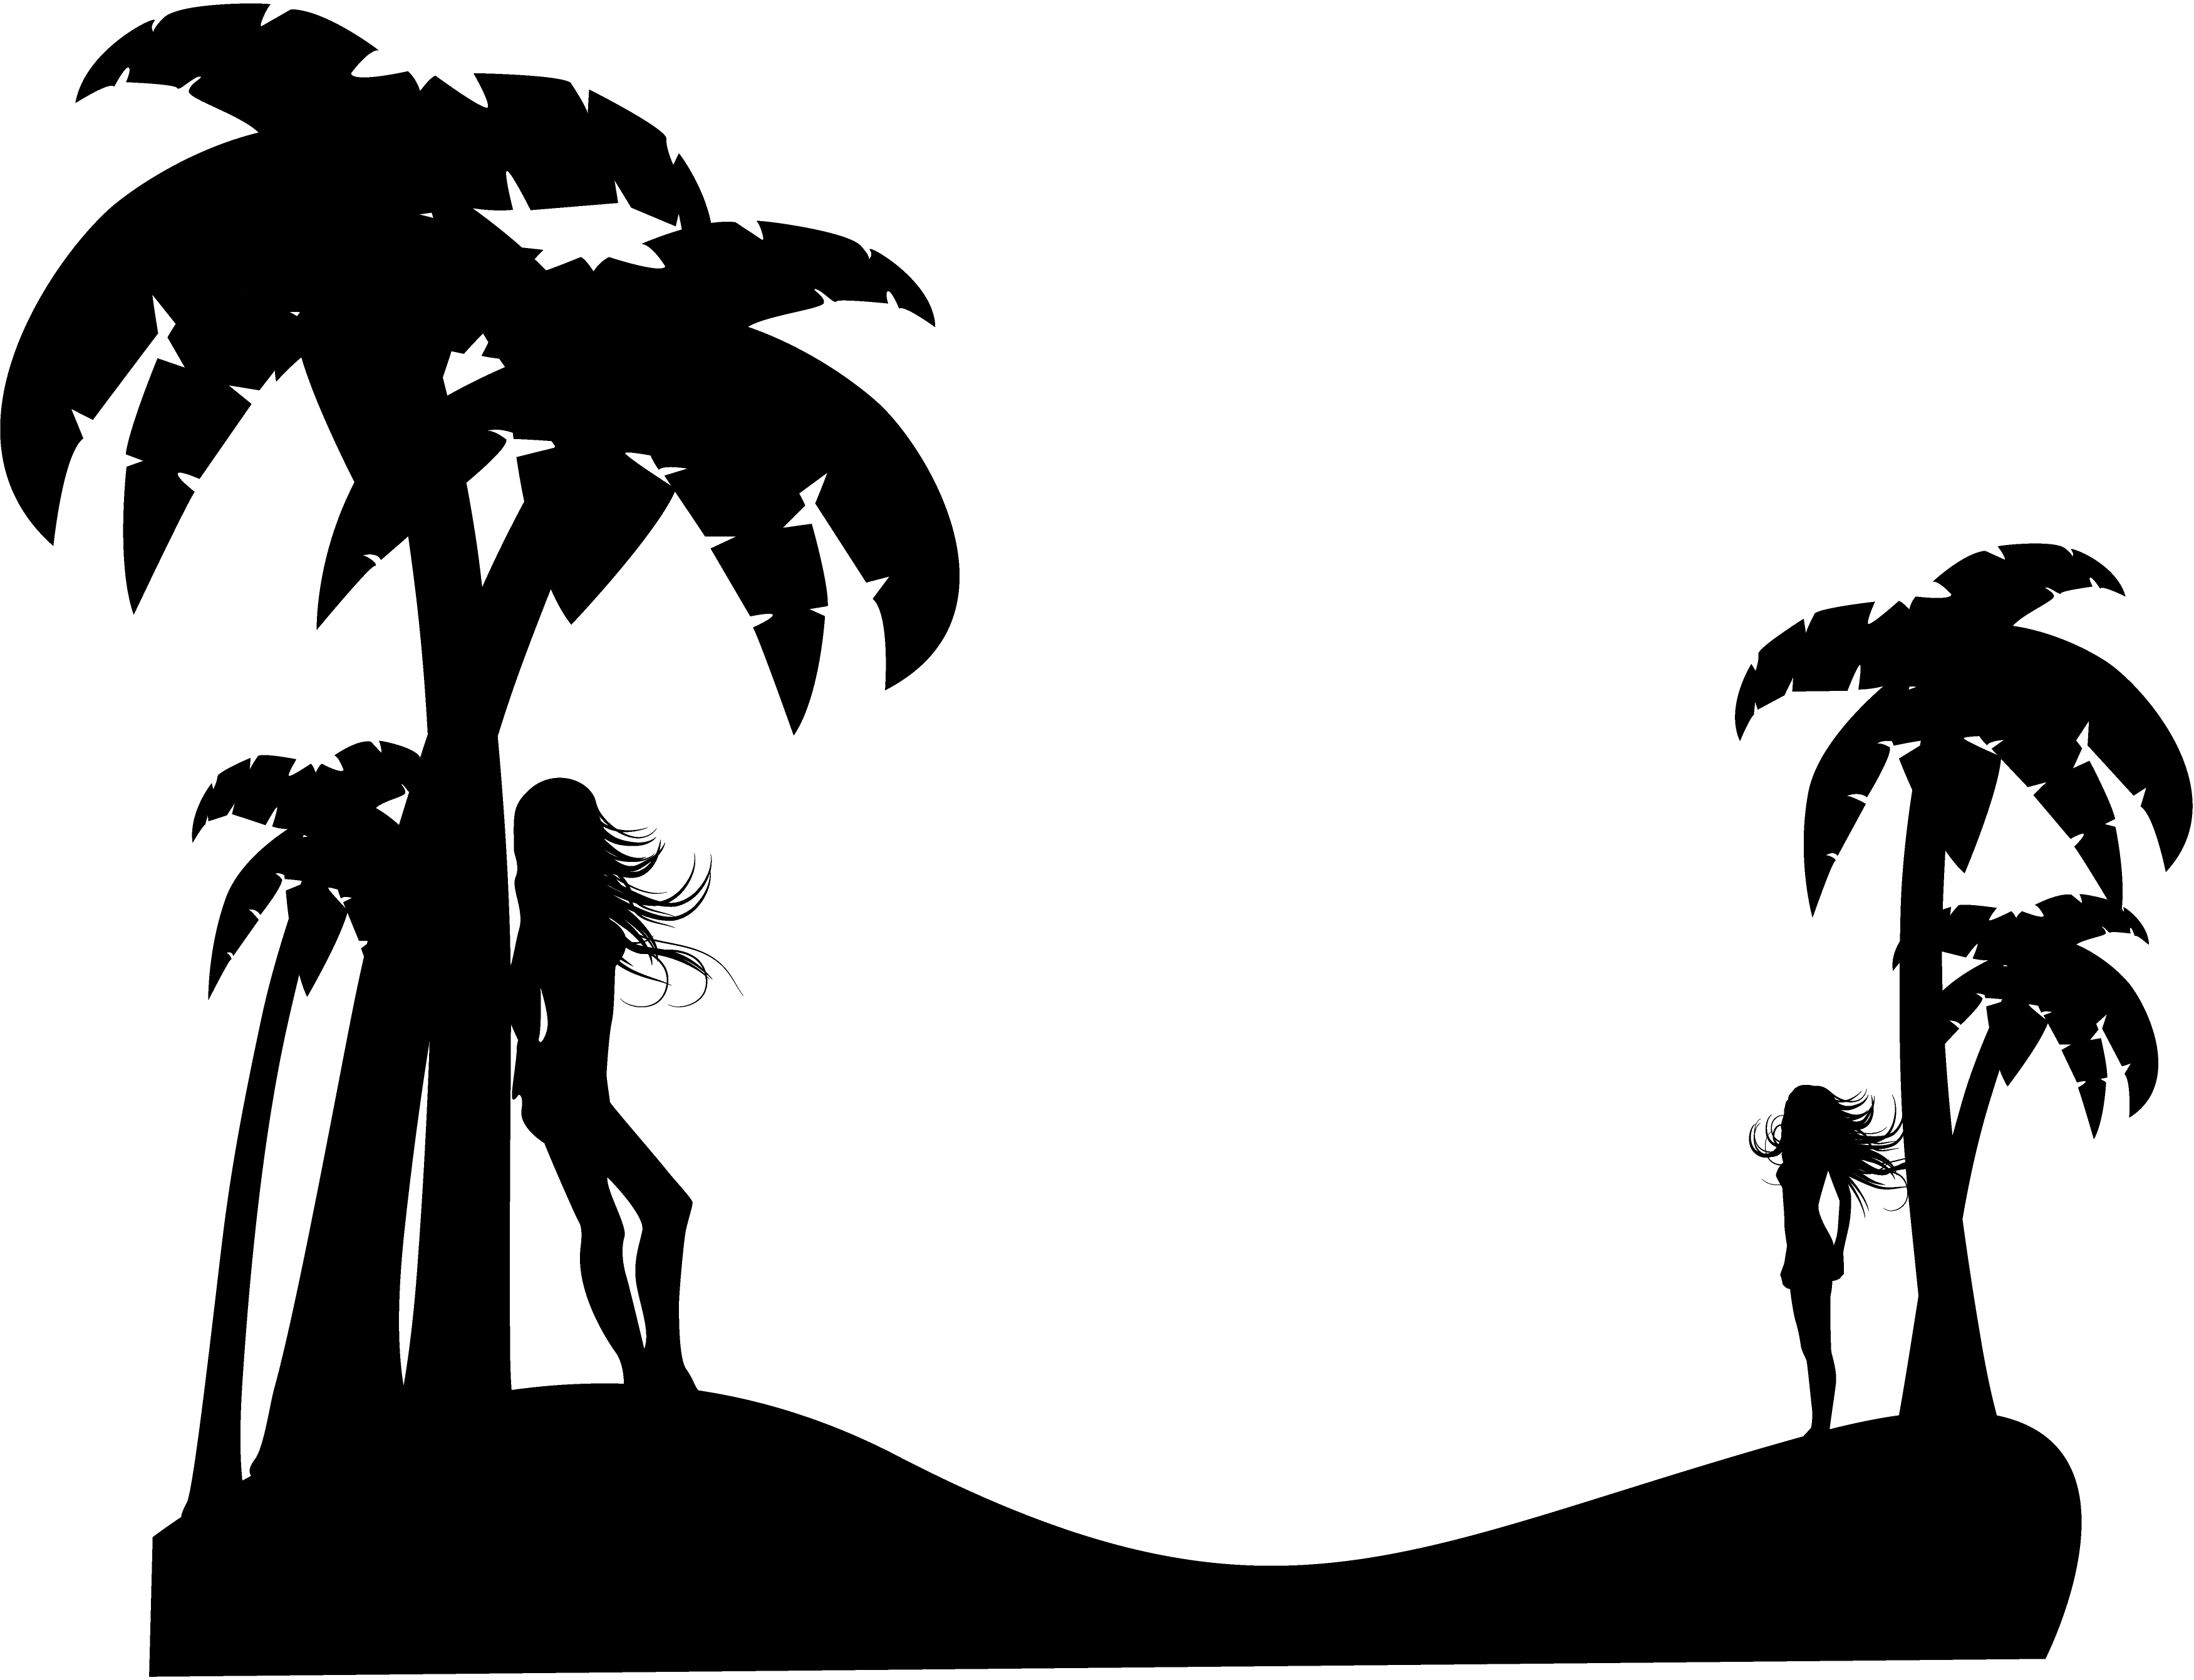
\includegraphics[width=0.8\textwidth]{wektor.jpg}
\caption{\label{fig:asda}}
\end{figure}

\end{document}